\documentclass[12pt]{article}
\usepackage{a4wide,bm,booktabs,graphicx,mathtools,hyperref,makecell,multirow,wasysym}
\usepackage[table]{xcolor}
\usepackage{blindtext}

\setlength{\parindent}{0pt}
\setlength{\parskip}{5pt plus 2pt minus 1pt}
\renewcommand{\arraystretch}{1.1}
\definecolor{ntc}{rgb}{0.58,0.11,0.5} % [148,27,128] / 255

\begin{document}

%%%%%%%%%%%%%%%%%%%%%%%%%%%%%%%%%%%%%%%%
% titlepage
\thispagestyle{empty}

\includegraphics[width=0.4\linewidth]{Figures/logo_NTC_en} \\

\begin{center}
{\large\it BIOMECHANICAL HUMAN BODY MODELS} \\ [5 mm]

\textcolor{ntc}{\hrule width \linewidth height 1pt} \vskip1cm

{\large\it SOFTWARE} \\ [5 mm]

{\bf Pelvic Floor Morphing} \\ [5 mm]

\textcolor{ntc}{\hrule width \linewidth height 1pt} \vskip1cm

\begin{tabular}{p{6cm} p{10cm}}
Author(s): & Lud\v{e}k Hyn\v{c}\'{\i}k, 61950 \\ [1 mm]
& Adam Wittek, The University of Western Australia \\
\end{tabular}

\vskip15mm

\begin{tabular} {p{6cm} p{10cm}}
Project number: & CZ.02.1.01/0.0/0.0/17\_048/0007280 \\
& Gledden fellowship, The University of Western Australia \\
\end{tabular}

\vskip15mm

\begin{tabular} {p{6cm} p{10cm}}
Report number: & NTC-ASW-26-001 \\ [2 mm]
Leader of department: & Jan Vychytil \\ [3 mm]
Director of centre: & Petr Kaval\'{\i}\v{r} \\
\end{tabular}

\vskip1cm

\textcolor{ntc}{\hrule width \linewidth height 1pt} \vskip1cm

{\large\it PLZE\v{N}, JUNE 2026}

\end{center}
\newpage

%%%%%%%%%%%%%%%%%%%%%%%%%%%%%%%%%%%%%%%%
\tableofcontents
\newpage
\setcounter{page}{1}

%%%%%%%%%%%%%%%%%%%%%%%%%%%%%%%%%%%%%%%%
\section*{Mathematical background}\addcontentsline{toc}{section}{\protect\numberline{}Mathematical background}
The aim of the software module is to register a reference model to a personalized model derived from subject-specific magnetic resonance imaging data.

The reference model is defined by a computational grid (nodes, which form elements). The \textbf{registration} is based on the corresponding \textbf{anatomical landmarks}, which are significant points on the biological tissues. The subject-specific anatomical landmarks corresponding to those defined on the reference model are acquired from the subject-specific medical images, e.g. magnetic resonance imaging (MRI), computer tomography (CT) or internal and external pelvimetry.

The registration updates the coordinates of the computational grid nodes to subject-specific computational grid nodes to create a personalised model by bringing closer the corresponding anatomical landmarks.

The registration of a reference model to a personalised model consists of 2 consecutive steps, particularly

\begin{enumerate}
\item \textbf{rigid registration}, which rotates and translates the coordinates of the reference computational grid nodes as close as possible to the position of the subject-specific magnetic resonance images by minimising the distance between the corresponding anatomical landmarks by means of the least squares method, and
\item \textbf{morphing}, which deforms the coordinates of the reference computational grid nodes to the position of the subject-specific magnetic resonance images by overlapping the coresponding anatomical landmarks.
\end{enumerate}

Consider the reference model computational grid with $n$ nodes and their coordinates ${\bf X}_i=\left[x_i,y_i,z_i\right]$, $i\in\{1,\dots,n\}$ in the matrix form

\begin{equation}
{\bf X}=\left[\begin{matrix}
x_1 & \dots & x_n \\
y_1 & \dots & y_n \\
z_1 & \dots & z_n\end{matrix}\right]
\end{equation}

where ${\bf X}$ is a $3\times n$ matrix. Consider $m$ corresponding landmarks on the reference model and the magnetic resonance images. Let's call the landmarks on the reference model ${\bf X}_{Lj}=\left[x_{Lj},y_{Lj},z_{Lj}\right]$, $j\in\{1,\dots,m\}$ as the \textit{baseline landmarks}, the reference model as the \textit{baseline model}, the subject-specific landmarks on the magnetic resonance images ${\bf X}_{Tj}=\left[x_{Tj},y_{Tj},z_{Tj}\right]$, $j\in\{1,\dots,m\}$ as the \textit{target landmarks} and the personalised model as the \textit{target model}.

In the text below, coordinates ${\bf X}$ corresponds to the reference model, coordinates $\widehat{\bf X}$ corresponds to the registered model and coordinates $\overline{\bf X}$ corresponds to the personalised model.

\subsection*{Rigid registration}\addcontentsline{toc}{subsection}{\protect\numberline{}Rigid registration}
The rigid registration rotates and translates the reference model to achieve the closest position to the subject-specific magnetic resonance images by the shortest distance between corresponding anatomical landmarks by means of the least square method. The {\bf Kabsch algorithm} is used for rigid registration.

\subsubsection*{Kabsch algoritm}\addcontentsline{toc}{subsubsection}{\protect\numberline{}Kabsch algoritm}
The Kabsch algoritm consisting of spatial rotation and translation minimizes root mean square deviation (RMSD). The aim is to find rotation $\bf R$ and translation $\bf t$ minimizing

\begin{equation}
\min_{{\bf R}, {\bf t}} \sum_{i=1}^{m} \| {\bf R}{\bf X}_{Li}+{\bf t}-{\bf X}_{Ti}\|^2
\end{equation}

where $\bf R$ is the spatial rotation matrix and $\bf t$ is the spatial translation vector. Firstly the centroids are calculated as 

\begin{equation}
{\bf P} = \frac{1}{m} \sum_{i=1}^m{\bf X}_{Li}, \quad
{\bf Q} = \frac{1}{m} \sum_{i=1}^m{\bf X}_{Ti}
\end{equation}

and all landmarks are centralized as

\begin{equation}
\widetilde{\bf X}_{L}={\bf X}_{L} - {\bf P}, \quad \widetilde{\bf X}_{T} = {\bf X}_{L}-{\bf Q}\mbox{.}
\end{equation}

Using the covariation matrix ${\bf H}=\widetilde{\bf X}_{L}^\top\widetilde{\bf X}_{T}$, the singular value decomposition is done as ${\bf H}={\bf U}{\bf\Sigma}{\bf V}^\top$. The optimum rotation is ${\bf R}={\bf V}{\bf U}^\top$. If $\det({\bf R})<0$, the mirroring is corrected as

\begin{equation}
{\bf V}[:, -1] \gets -{\bf V}[:, -1], \quad {\bf R}={\bf V}{\bf U}^\top\mbox{.}
\end{equation}

The translation is calculated as ${\bf t}={\bf Q}-{\bf R}{\bf P}$. Finally, the registered points are calculated as $\widehat{\bf X}_i={\bf X}_i+{\bf t}$, $i\in\{1,\dots,n\}$, and $\widehat{\bf X}_{Lj}={\bf X}_{Lj}+{\bf t}$, $j\in\{1,\dots,m\}$.

\subsection*{Morphing}\addcontentsline{toc}{subsection}{\protect\numberline{}Morphing}
The morphing deforms the rigidly registered reference model (defined by grid nodes coordinates~$\widehat{\bf X}$) to the position of the subject-specific magnetic resonance images to create a personalised model (defined by target computational grid nodes coordinates $\overline{\bf X}$) by interpolation using {\bf radial basis function}.

\subsubsection*{Radial basis function}\addcontentsline{toc}{subsubsection}{\protect\numberline{}Radial basis function}
Radial basis functions (RBF) to interpolate function $g({\bf X})$ at the point ${\bf X}$ having $m$ landmarks on both the baseline and the target grids takes the form~\cite{Carr:2007}

\begin{equation}
\label{interpolation}
g({\bf X})=p({\bf X})+\sum\limits_{j=1}^m\lambda_j\varphi\left(\|{\bf X}-{\bf X}_j\|\right)+\alpha
\end{equation}

where $p({\bf X})$ is a low order polynomial, $\lambda_j$, $j\in\{1,\dots,m\}$, is the weighting coefficient, $\varphi$ is the radial basis function, $\|{\bf X}-{\bf X}_j\|=\sqrt{(x-x_j)^2+(y-y_j)^2+(z-z_j)^2}$ and $\alpha$ is a constant. The first order polynomial selected for $p({\bf X})=\left[1,x,y,z\right]\left[c_0,c_1,c_2,c_3\right]^{\mathrm{T}}={\bf X}{\bf c}$ and $\varphi$ is the radial basis function.

Substituting the rigidly registered baseline landmarks $\left[\widehat{x}_{Lj},\widehat{y}_{Lj},\widehat{z}_{Lj}\right]=\widehat{\bf X}_{Lj}$, $j\in\{1,\dots,m\}$ and the target landmarks $f({\bf X})=\left[x_{Ti},y_{Ti},z_{Ti}\right]={\bf X}_{Ti}$, $j\in\{1,\dots,m\}$ to Equation (\ref{interpolation}) brings

\begin{equation}
{\bf X}_{Ti}=\sum\limits_{j=1}^m\lambda_j\varphi\left(\|\widehat{\bf X}_{Li}-{\bf X}_{Tj}\|\right)+\alpha+\widehat{\bf X}_{Li}{\bf c}\mbox{,}\quad j\in\{1,\dots,m\}
\end{equation}

or

\begin{equation}
\label{RBF}
\left[\begin{matrix}
{\bf A}+\alpha{\bf I} & {\bf B}\\[1ex]
%{\bf A} & {\bf B}\\[1ex]
{\bf B}^{\mathrm{T}} & {\bf 0}
\end{matrix}\right]
\left[\begin{matrix}
\bm\lambda\\[1ex]
{\bf c}
\end{matrix}\right]=
\left[\begin{matrix}
{\bf T}\\[1ex]
{\bf 0}
\end{matrix}\right]
\end{equation}

in the matrix form, where matrix ${\bf A}=A_{ij}=\varphi\left(r_{ij}\right)$ is a square $m\times m$ matrix containing the distances between the mutual pairs of the baseline landmarks $r_{ij}=\|\widehat{\bf X}_{Li}-\widehat{\bf X}_{Lj}\|$, $\forall i,j\in\{1,\dots,m\}$, ${\bf I}$ is the identity matrix of size $m\times m$,

\begin{equation}
{\bf B}=\left[\begin{matrix}
1 & \widehat{x}_{L1} & \widehat{y}_{L1} & \widehat{z}_{L1}\\
\vdots & \vdots & \vdots & \vdots\\
1 & \widehat{x}_{Lm} & \widehat{y}_{Lm} & \widehat{z}_{Lm}
\end{matrix}\right]
\end{equation}

is a $m\times 4$ matrix containing the coordinates of the baseline landmarks, 

\begin{equation}
{\bf T}=\left[\begin{matrix}
{x}_{T1} & \dots & {x}_{Tm} \\
{y}_{T1} & \dots & {y}_{Tm} \\
{z}_{T1} & \dots & {z}_{Tm}
\end{matrix}\right]
\end{equation}

is a $3\times m$ matrix containing the coordinates of the target landmarks and ${\bf c}$ is constant matrix. Solving Equation (\ref{RBF}) brings the matrix $\bm\lambda$ of size $m\times 3$ and the matrix ${\bf c}$ of size $4\times 3$. Once they are determined, by assuming that the number of nodes in the baseline grid is $n$, the coordinates of the nodes in morphed grid $\overline{\bf X}$ (a matrix of size $n\times 3$) can be calculated as

\begin{equation}
\left[\begin{matrix}
\overline{\bf X}\\[1ex]
{\bf 0}
\end{matrix}\right]
=
\left[\begin{matrix}
%\overline{\bf A}+\alpha{\bf I} & \overline{\bf B}\\[1ex]
\overline{\bf A} & \overline{\bf B}\\[1ex]
{\bf B}^{\mathrm{T}} & {\bf 0}
\end{matrix}\right]
\left[\begin{matrix}
\bm\lambda\\[1ex]
{\bf c}
\end{matrix}\right]
\end{equation}

where

\begin{equation}
\overline{\bf X}=\left[\begin{matrix}
\overline{x}_1 & \overline{y}_1 & \overline{z}_1\\
\vdots & \vdots & \vdots\\
\overline{x}_n & \overline{y}_n & \overline{z}_n
\end{matrix}\right]
\end{equation}

is a $n\times 3$ matrix containing the coordinates of the nodes in the morphed grid, matrix $\overline{\bf A}=\overline{A}_{ij}=\varphi\left(r_{ij}\right)$ is a $n\times m$ matrix, where $i\in\{1,\dots,n\}$ are the nodes in the baseline grid, $j\in\{1,\dots,m\}$ are the baseline landmarks and

\begin{equation}
\overline{\bf B}=\left[\begin{matrix}
1 & \widehat{x}_1 & \widehat{y}_1 & \widehat{z}_1\\
\vdots & \vdots & \vdots & \vdots\\
1 & \widehat{x}_n & \widehat{y}_n & \widehat{z}_n
\end{matrix}\right]
\end{equation}

is a $n\times 4$ matrix containing the coordinates of the nodes in the baseline grid. The radial basis function can be chosen either

\begin{itemize}
\item \textbf{thin plate spline}~\cite{Skala:2016}, which has a global support and is defined as 

\begin{equation}
\varphi(r)=r^2\log{r}
\end{equation}

where $r=\|{\bf X}-{\bf X}_i\|$, which generally results in a smooth mesh~\cite{Hwang:2016}, or
\item \textbf{Wendland C2 compact support function}~\cite{Wendland:1995}, which has a local support, is $C^2$-smooth and is useful for morphing in biomechanics. It is defined as

\begin{equation}
\varphi(r) = 
\begin{cases} 
(1 - r)^4 \,(4 r + 1), & 0 \le r \le 1, \\
0, & r > 1,
\end{cases}
\end{equation}

where $r = \frac{\|{\bf X}-{\bf X}_i\|}{R}$ and $R$ is the support radius.
\end{itemize}


%%%%%%%%%%%%%%%%%%%%%%%%%%%%%%%%%%%%%%%%
\newpage
\section*{Implementation}\addcontentsline{toc}{section}{\protect\numberline{}Implementation}
The software module concerns the 2026 version of 3D Slicer extension {\it Pelvic Floor model} (PelFoM) available at \href{https://github.com/PelFoM}{GitHub}, see Figure \ref{fig:environment}. 

\begin{figure}[h]
\centering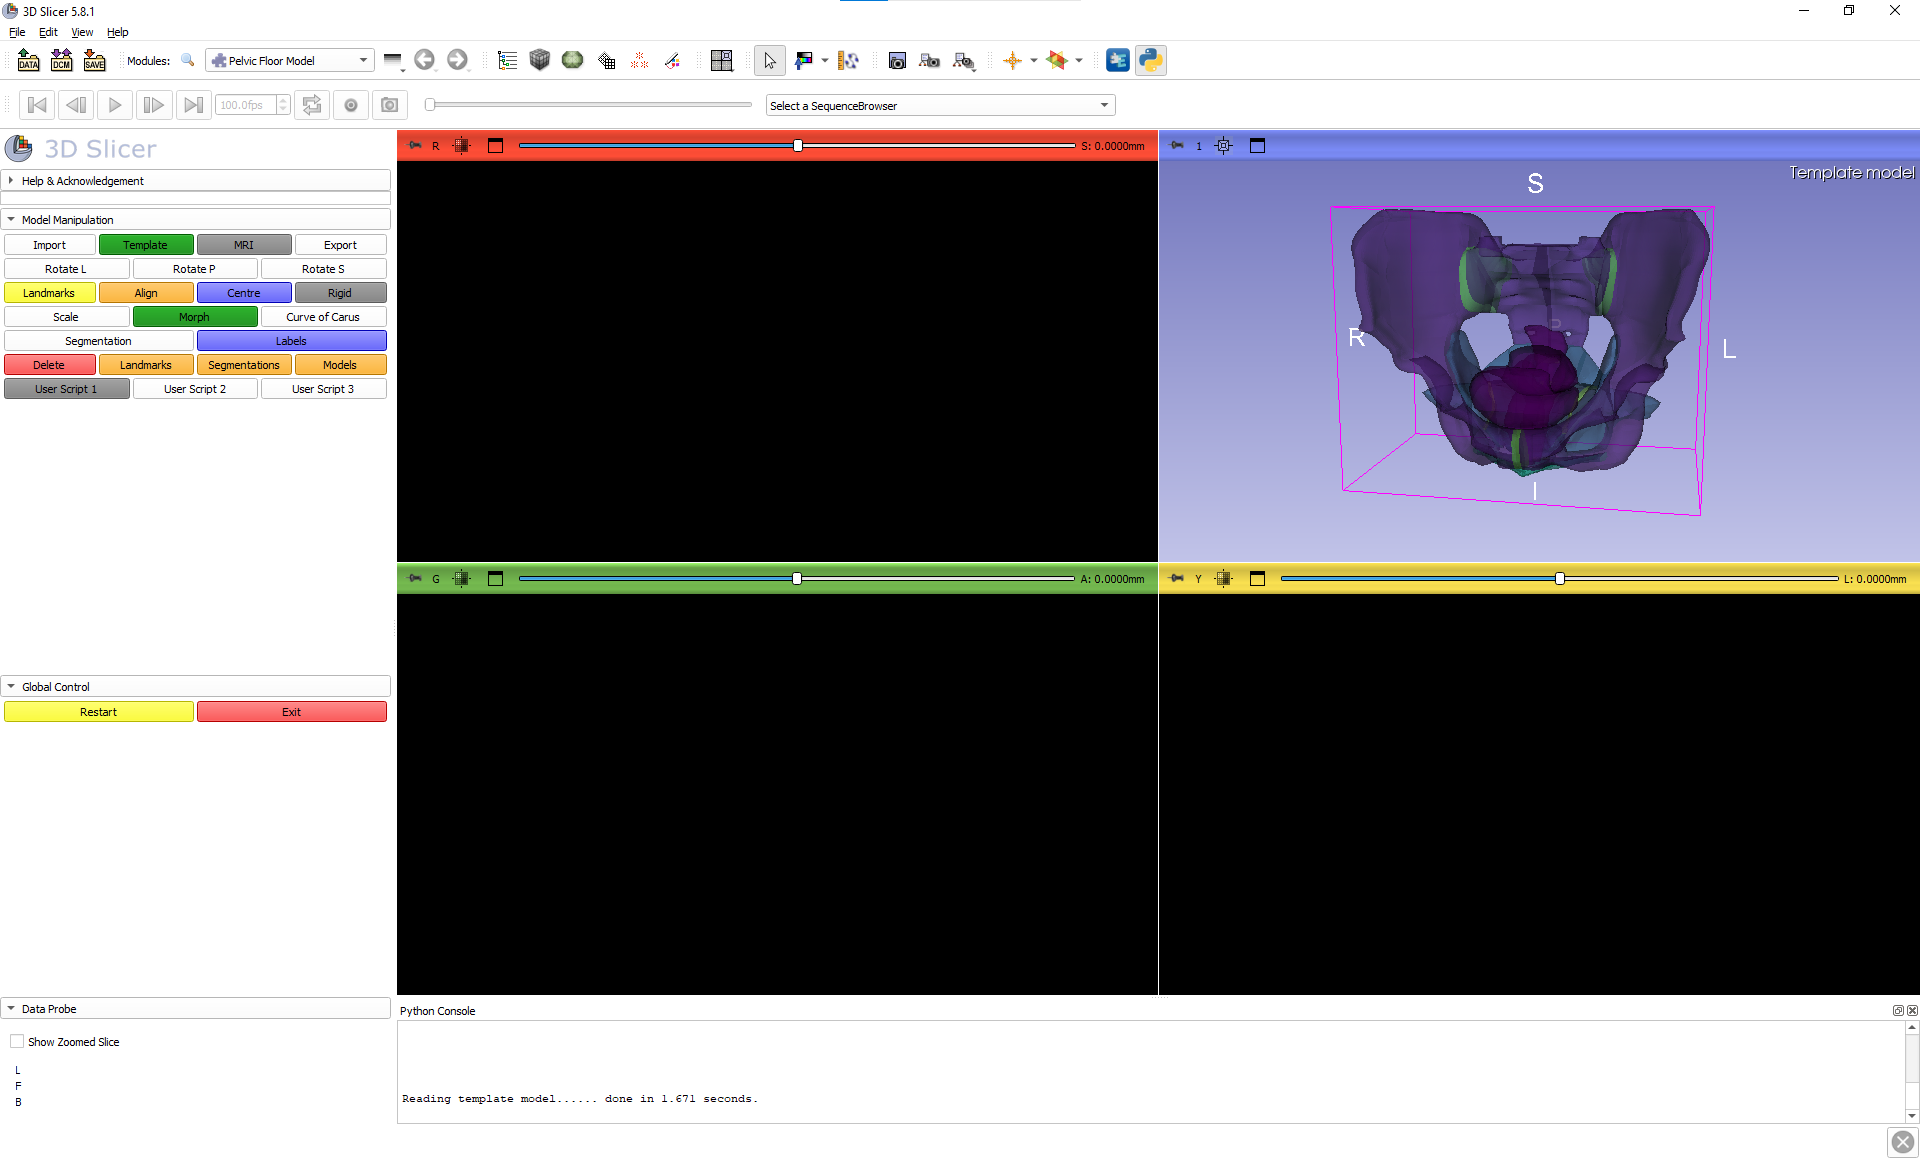
\includegraphics[width=\textwidth]{Figures/environment}
\caption{Environment eith the reference model}\label{fig:environment}
\end{figure}

%%%%%%%%%%%%%%%%%%%%%%%%%%%%%%%%%%%%%%%%
\subsection*{License}\addcontentsline{toc}{subsection}{\protect\numberline{}License}
The module is available under a BSD 3-Clause "New" or "Revised" License.

\subsection*{Installation}\addcontentsline{toc}{subsection}{\protect\numberline{}Installation}
For installation, follow the steps in the \href{https://docs.google.com/presentation/d/1jcyetWDrEB9OtRtLg6uCvz5_fK_u3cEZl25lYEZmLOw/present}{Installation Manual}. Developers may use \href{https://docs.google.com/spreadsheets/d/1wAweZy6TkhwOCEfc8A3dBSrNZwW-ndznlEXvNUEGGFk/edit}{Developers Manual} and \href{https://docs.google.com/presentation/d/1aj0amaTXFlie0vdCJsjmK7jthto73RxiStYDiB6T8uw/present}{Code Structure}. The mathematical theory of registration is described here and available \href{https://github.com/PelFoM/Theory/blob/main/Pelvic_Floor_Morphing.pdf}{online}.

%%%%%%%%%%%%%%%%%%%%%%%%%%%%%%%%%%%%%%%%
\subsection*{Reference model}\addcontentsline{toc}{subsection}{\protect\numberline{}Reference model}
The module consists of a reference bony pelvis model (see Figure \ref{fig:environment}) including pre-defined anatomical landmarks (see Table \ref{tab:landmarks} and Figure \ref{fig:landmarks}).

%%%%%%%%%%%%%%%%%%%%%%%%%%%%%%%%%%%%%%%%
\subsubsection*{Anatomical landmarks}\addcontentsline{toc}{subsubsection}{\protect\numberline{}Anatomical landmarks}
\begin{table}[h]
\centering\begin{tabular}{|l|l|}
\hline
\textbf{Landmark} & \textbf{Anatomical description} \\
\hline
PSA & Anterior point of the pubic symphysis (superior border) \\
PSP & Posterior point of the pubic symphysis \\
PSI & Inferior point of the pubic symphysis (inferior border) \\
L5 & Spinous process of the fifth lumbar vertebra \\
PR & Sacral promontory \\
S3 & Midpoint of the superior surface of the third sacral vertebra (S3) \\
SJ & Sacrococcygeal joint (internal landmark) \\
SB & Sacrococcygeal joint (external surface landmark) \\
ILL & Left-most point on the iliopectineal line \\
ILR & Right-most point on the iliopectineal line \\
BCL & Left iliac crest (distantia bicristalis) \\
BCR & Right iliac crest (distantia bicristalis) \\
BSL & Left anterior superior iliac spine (distantia bispinalis) \\
BSR & Right anterior superior iliac spine (distantia bispinalis) \\
ISL & Left ischial spine \\
ISR & Right ischial spine \\
ITL & Left ischial tuberosity \\
ITR & Right ischial tuberosity \\
TIL & Left tuber ischiadicum \\
TIR & Right tuber ischiadicum \\
PSISL & Left posterior superior iliac spine (skin dimple) \\
PSISR & Right posterior superior iliac spine (skin dimple) \\
TRL & Left greater trochanter \\
TRR & Right greater trochanter \\
\hline
\end{tabular}
\caption{Anatomical landmarks}\label{tab:landmarks}
\end{table}

\begin{figure}[h]
\centering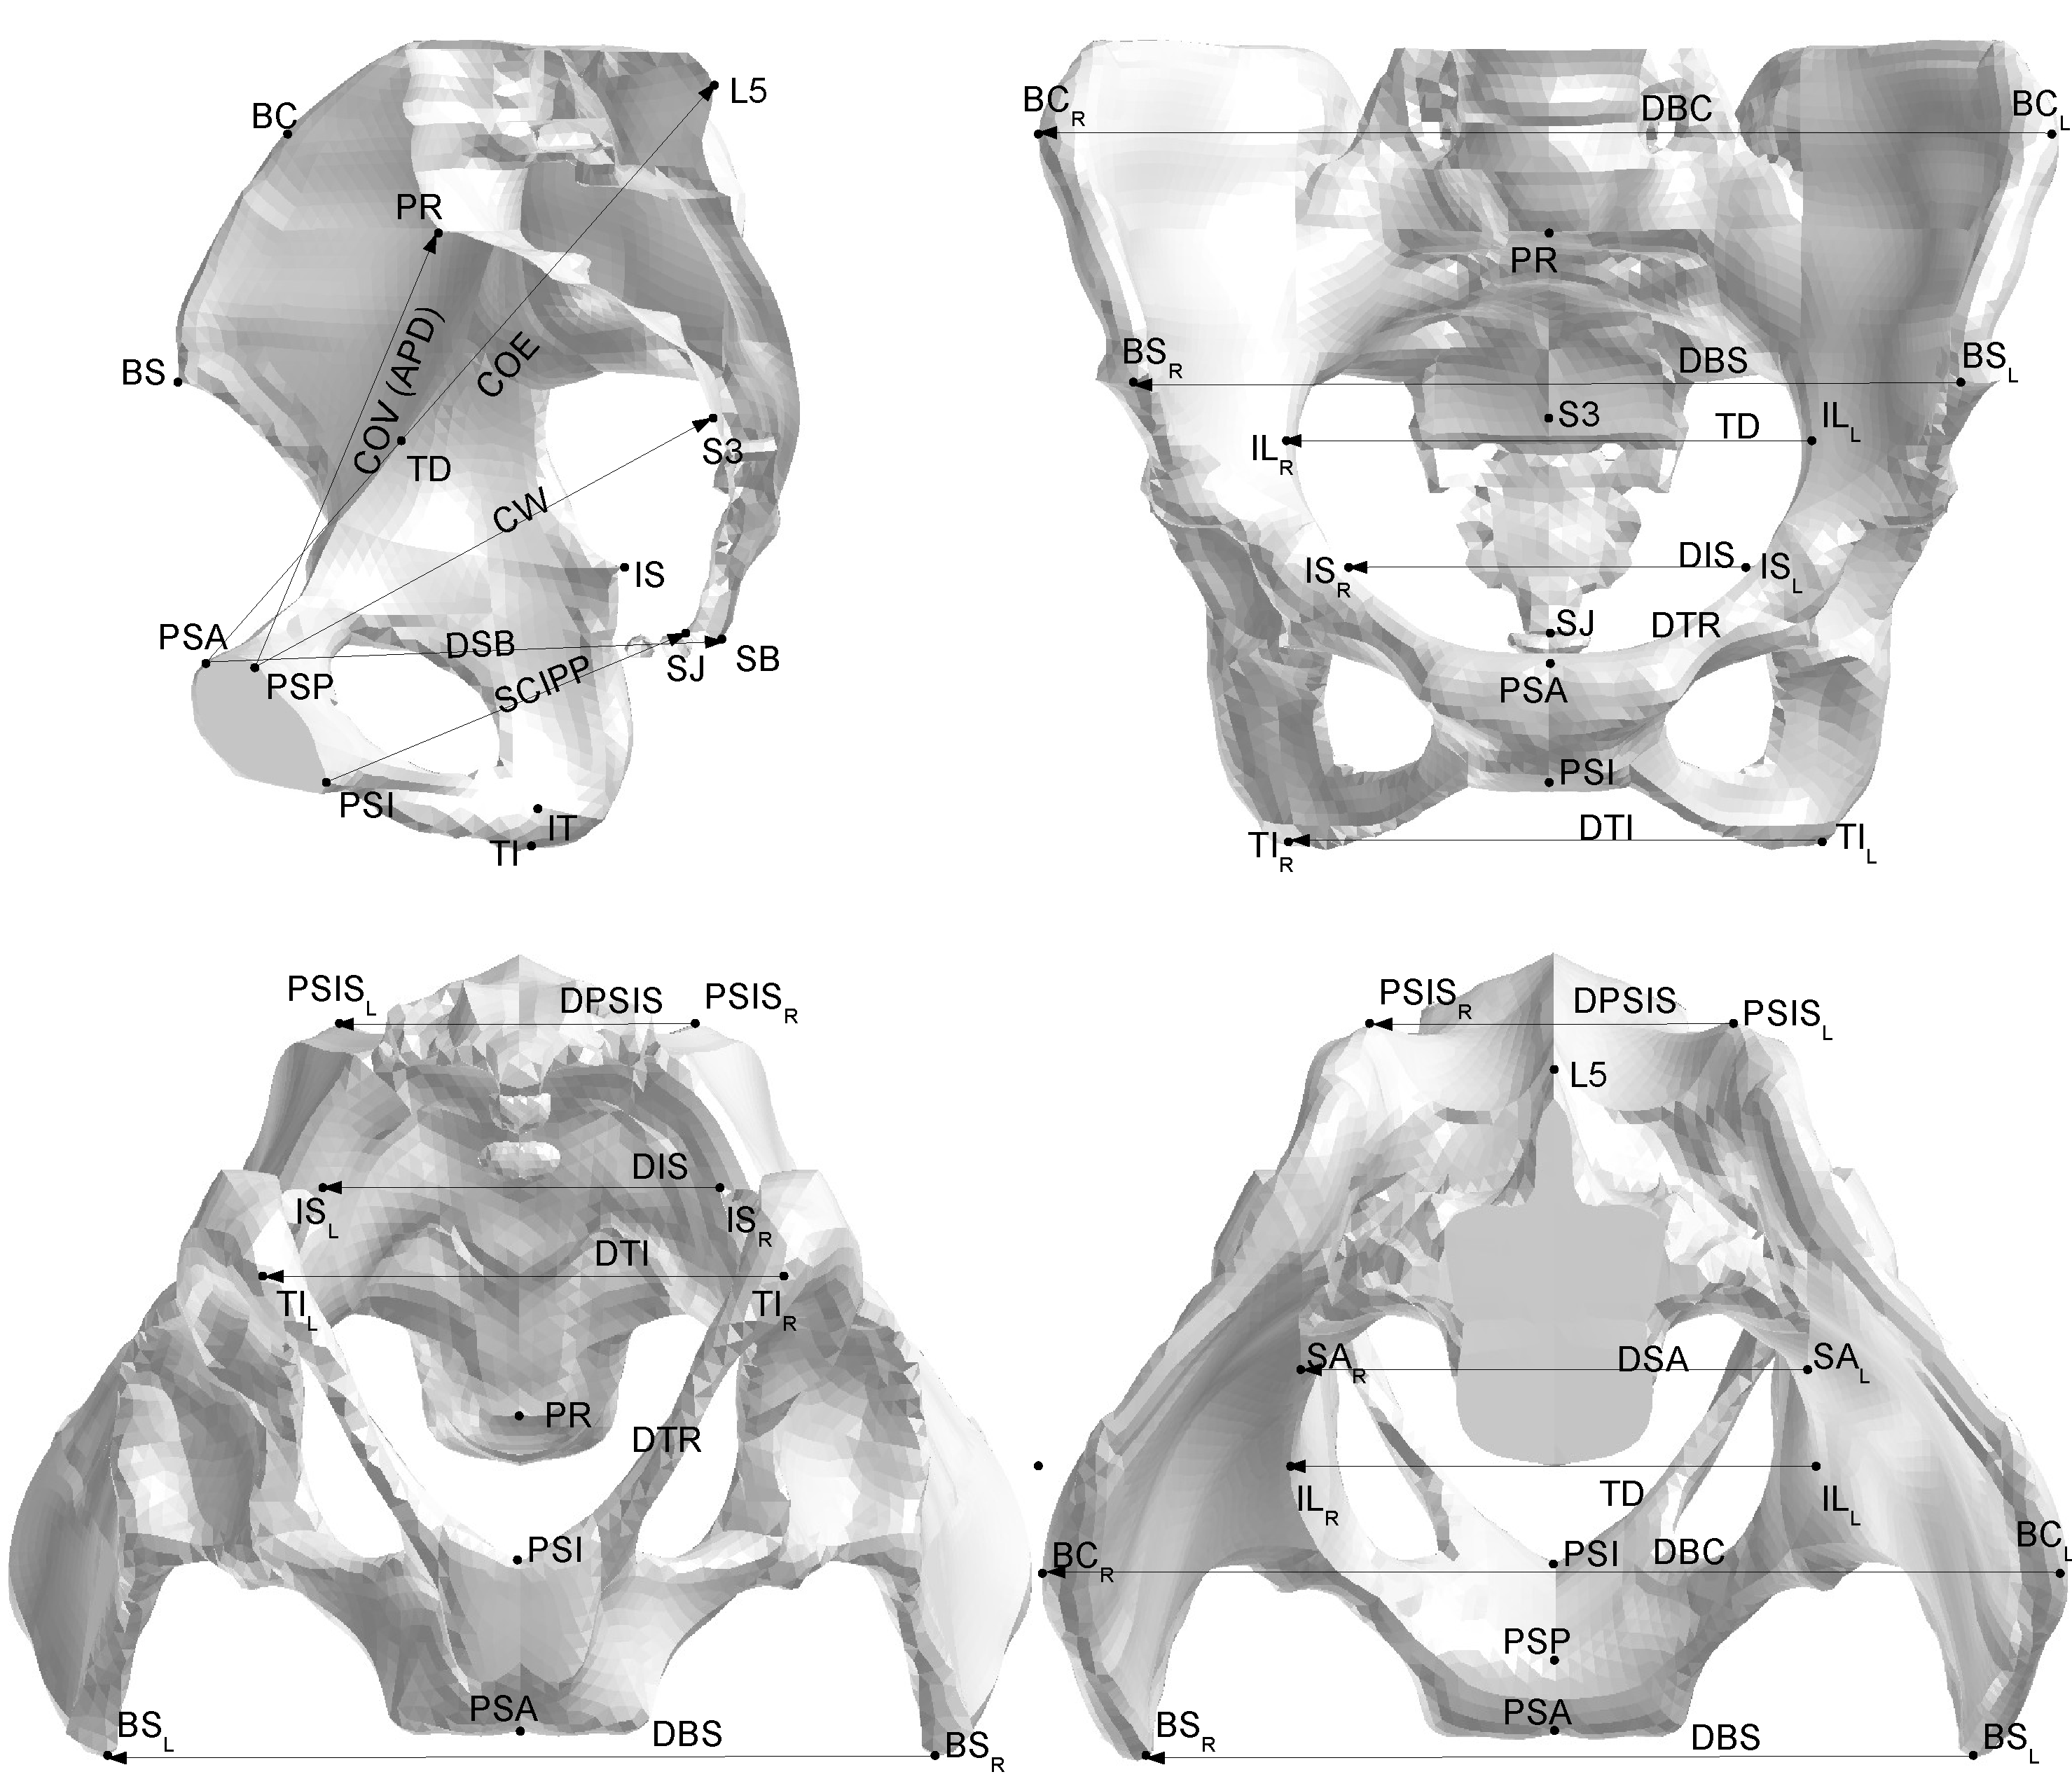
\includegraphics[width=0.9\textwidth]{Pelvimetry/pelvimetry}
\caption{Anatomical landmarks}\label{fig:landmarks}
\end{figure}

%%%%%%%%%%%%%%%%%%%%%%%%%%%%%%%%%%%%%%%%
\section*{Acknowledgement}\addcontentsline{toc}{section}{\protect\numberline{}Acknowledgement}
The work was supported by the project "Integration of biomedical research and health care in the Pilsen metropolitan area“; reg. no. CZ.02.01.01/00/23\_021/0008828) - co-funded by the European Union and by the State Budget of the Czech Republic.

%%%%%%%%%%%%%%%%%%%%%%%%%%%%%%%%%%%%%%%%
\bibliographystyle{plain}\addcontentsline{toc}{section}{\protect\numberline{}References} 
\bibliography{bibliography}

\end{document}
